\documentclass[11pt]{article}

    \usepackage[breakable]{tcolorbox}
    \usepackage{parskip} % Stop auto-indenting (to mimic markdown behaviour)
    
    \usepackage{iftex}
    \ifPDFTeX
    	\usepackage[T1]{fontenc}
    	\usepackage{mathpazo}
    \else
    	\usepackage{fontspec}
    \fi

    % Basic figure setup, for now with no caption control since it's done
    % automatically by Pandoc (which extracts ![](path) syntax from Markdown).
    \usepackage{graphicx}
    % Maintain compatibility with old templates. Remove in nbconvert 6.0
    \let\Oldincludegraphics\includegraphics
    % Ensure that by default, figures have no caption (until we provide a
    % proper Figure object with a Caption API and a way to capture that
    % in the conversion process - todo).
    \usepackage[font=scriptsize]{caption}
    % \DeclareCaptionFormat{nocaption}{}
    % \captionsetup{format=nocaption,aboveskip=0pt,belowskip=0pt}

    \usepackage[Export]{adjustbox} % Used to constrain images to a maximum size
    \adjustboxset{max size={0.9\linewidth}{0.9\paperheight}}
    \usepackage{float}
    \floatplacement{figure}{H} % forces figures to be placed at the correct location
    \usepackage{xcolor} % Allow colors to be defined
    \usepackage{enumerate} % Needed for markdown enumerations to work
    \usepackage{geometry} % Used to adjust the document margins
    \usepackage{amsmath} % Equations
    \usepackage{amssymb} % Equations
    \usepackage{textcomp} % defines textquotesingle
    % Hack from http://tex.stackexchange.com/a/47451/13684:
    \AtBeginDocument{%
        \def\PYZsq{\textquotesingle}% Upright quotes in Pygmentized code
    }
    \usepackage{upquote} % Upright quotes for verbatim code
    \usepackage{eurosym} % defines \euro
    \usepackage[mathletters]{ucs} % Extended unicode (utf-8) support
    \usepackage{fancyvrb} % verbatim replacement that allows latex
    \usepackage{grffile} % extends the file name processing of package graphics 
                         % to support a larger range
    \makeatletter % fix for grffile with XeLaTeX
    \def\Gread@@xetex#1{%
      \IfFileExists{"\Gin@base".bb}%
      {\Gread@eps{\Gin@base.bb}}%
      {\Gread@@xetex@aux#1}%
    }
    \makeatother

    % The hyperref package gives us a pdf with properly built
    % internal navigation ('pdf bookmarks' for the table of contents,
    % internal cross-reference links, web links for URLs, etc.)
    \usepackage{hyperref}
    % The default LaTeX title has an obnoxious amount of whitespace. By default,
    % titling removes some of it. It also provides customization options.
    \usepackage{titling}
    \setlength{\droptitle}{-2cm}
    \usepackage{longtable} % longtable support required by pandoc >1.10
    \usepackage{booktabs}  % table support for pandoc > 1.12.2
    \usepackage[inline]{enumitem} % IRkernel/repr support (it uses the enumerate* environment)
    \usepackage[normalem]{ulem} % ulem is needed to support strikethroughs (\sout)
                                % normalem makes italics be italics, not underlines
    \usepackage{mathrsfs}
    

    
    % Colors for the hyperref package
    \definecolor{urlcolor}{rgb}{0,.145,.698}
    \definecolor{linkcolor}{rgb}{.71,0.21,0.01}
    \definecolor{citecolor}{rgb}{.12,.54,.11}

    % ANSI colors
    \definecolor{ansi-black}{HTML}{3E424D}
    \definecolor{ansi-black-intense}{HTML}{282C36}
    \definecolor{ansi-red}{HTML}{E75C58}
    \definecolor{ansi-red-intense}{HTML}{B22B31}
    \definecolor{ansi-green}{HTML}{00A250}
    \definecolor{ansi-green-intense}{HTML}{007427}
    \definecolor{ansi-yellow}{HTML}{DDB62B}
    \definecolor{ansi-yellow-intense}{HTML}{B27D12}
    \definecolor{ansi-blue}{HTML}{208FFB}
    \definecolor{ansi-blue-intense}{HTML}{0065CA}
    \definecolor{ansi-magenta}{HTML}{D160C4}
    \definecolor{ansi-magenta-intense}{HTML}{A03196}
    \definecolor{ansi-cyan}{HTML}{60C6C8}
    \definecolor{ansi-cyan-intense}{HTML}{258F8F}
    \definecolor{ansi-white}{HTML}{C5C1B4}
    \definecolor{ansi-white-intense}{HTML}{A1A6B2}
    \definecolor{ansi-default-inverse-fg}{HTML}{FFFFFF}
    \definecolor{ansi-default-inverse-bg}{HTML}{000000}

    % commands and environments needed by pandoc snippets
    % extracted from the output of `pandoc -s`
    \providecommand{\tightlist}{%
      \setlength{\itemsep}{0pt}\setlength{\parskip}{0pt}}
    \DefineVerbatimEnvironment{Highlighting}{Verbatim}{commandchars=\\\{\},numbers=left,fontsize=\small}
    % Add ',fontsize=\small' for more characters per line
    \newenvironment{Shaded}{}{}
    \newcommand{\KeywordTok}[1]{\textcolor[rgb]{0.00,0.44,0.13}{\textbf{{#1}}}}
    \newcommand{\DataTypeTok}[1]{\textcolor[rgb]{0.56,0.13,0.00}{{#1}}}
    \newcommand{\DecValTok}[1]{\textcolor[rgb]{0.25,0.63,0.44}{{#1}}}
    \newcommand{\BaseNTok}[1]{\textcolor[rgb]{0.25,0.63,0.44}{{#1}}}
    \newcommand{\FloatTok}[1]{\textcolor[rgb]{0.25,0.63,0.44}{{#1}}}
    \newcommand{\CharTok}[1]{\textcolor[rgb]{0.25,0.44,0.63}{{#1}}}
    \newcommand{\StringTok}[1]{\textcolor[rgb]{0.25,0.44,0.63}{{#1}}}
    \newcommand{\CommentTok}[1]{\textcolor[rgb]{0.38,0.63,0.69}{\textit{{#1}}}}
    \newcommand{\OtherTok}[1]{\textcolor[rgb]{0.00,0.44,0.13}{{#1}}}
    \newcommand{\AlertTok}[1]{\textcolor[rgb]{1.00,0.00,0.00}{\textbf{{#1}}}}
    \newcommand{\FunctionTok}[1]{\textcolor[rgb]{0.02,0.16,0.49}{{#1}}}
    \newcommand{\RegionMarkerTok}[1]{{#1}}
    \newcommand{\ErrorTok}[1]{\textcolor[rgb]{1.00,0.00,0.00}{\textbf{{#1}}}}
    \newcommand{\NormalTok}[1]{{#1}}
    
    % Additional commands for more recent versions of Pandoc
    \newcommand{\ConstantTok}[1]{\textcolor[rgb]{0.53,0.00,0.00}{{#1}}}
    \newcommand{\SpecialCharTok}[1]{\textcolor[rgb]{0.25,0.44,0.63}{{#1}}}
    \newcommand{\VerbatimStringTok}[1]{\textcolor[rgb]{0.25,0.44,0.63}{{#1}}}
    \newcommand{\SpecialStringTok}[1]{\textcolor[rgb]{0.73,0.40,0.53}{{#1}}}
    \newcommand{\ImportTok}[1]{{#1}}
    \newcommand{\DocumentationTok}[1]{\textcolor[rgb]{0.73,0.13,0.13}{\textit{{#1}}}}
    \newcommand{\AnnotationTok}[1]{\textcolor[rgb]{0.38,0.63,0.69}{\textbf{\textit{{#1}}}}}
    \newcommand{\CommentVarTok}[1]{\textcolor[rgb]{0.38,0.63,0.69}{\textbf{\textit{{#1}}}}}
    \newcommand{\VariableTok}[1]{\textcolor[rgb]{0.10,0.09,0.49}{{#1}}}
    \newcommand{\ControlFlowTok}[1]{\textcolor[rgb]{0.00,0.44,0.13}{\textbf{{#1}}}}
    \newcommand{\OperatorTok}[1]{\textcolor[rgb]{0.40,0.40,0.40}{{#1}}}
    \newcommand{\BuiltInTok}[1]{{#1}}
    \newcommand{\ExtensionTok}[1]{{#1}}
    \newcommand{\PreprocessorTok}[1]{\textcolor[rgb]{0.74,0.48,0.00}{{#1}}}
    \newcommand{\AttributeTok}[1]{\textcolor[rgb]{0.49,0.56,0.16}{{#1}}}
    \newcommand{\InformationTok}[1]{\textcolor[rgb]{0.38,0.63,0.69}{\textbf{\textit{{#1}}}}}
    \newcommand{\WarningTok}[1]{\textcolor[rgb]{0.38,0.63,0.69}{\textbf{\textit{{#1}}}}}
    
    
    % Define a nice break command that doesn't care if a line doesn't already
    % exist.
    \def\br{\hspace*{\fill} \\* }
    % Math Jax compatibility definitions
    \def\gt{>}
    \def\lt{<}
    \let\Oldtex\TeX
    \let\Oldlatex\LaTeX
    \renewcommand{\TeX}{\textrm{\Oldtex}}
    \renewcommand{\LaTeX}{\textrm{\Oldlatex}}
    % Document parameters
    % Document title
    
\title{COVID-19: perché si effettuano due o più test? Quanti test sono necessari per ritenere infetto, sano o guarito un individuo?}

    
    
\author{Max Pierini}
\date{%
    \href{mailto:info@maxpierini.it}{info@maxpierini.it}\\%
    \today
}

    
% Pygments definitions
\makeatletter
\def\PY@reset{\let\PY@it=\relax \let\PY@bf=\relax%
    \let\PY@ul=\relax \let\PY@tc=\relax%
    \let\PY@bc=\relax \let\PY@ff=\relax}
\def\PY@tok#1{\csname PY@tok@#1\endcsname}
\def\PY@toks#1+{\ifx\relax#1\empty\else%
    \PY@tok{#1}\expandafter\PY@toks\fi}
\def\PY@do#1{\PY@bc{\PY@tc{\PY@ul{%
    \PY@it{\PY@bf{\PY@ff{#1}}}}}}}
\def\PY#1#2{\PY@reset\PY@toks#1+\relax+\PY@do{#2}}

\expandafter\def\csname PY@tok@w\endcsname{\def\PY@tc##1{\textcolor[rgb]{0.73,0.73,0.73}{##1}}}
\expandafter\def\csname PY@tok@c\endcsname{\let\PY@it=\textit\def\PY@tc##1{\textcolor[rgb]{0.25,0.50,0.50}{##1}}}
\expandafter\def\csname PY@tok@cp\endcsname{\def\PY@tc##1{\textcolor[rgb]{0.74,0.48,0.00}{##1}}}
\expandafter\def\csname PY@tok@k\endcsname{\let\PY@bf=\textbf\def\PY@tc##1{\textcolor[rgb]{0.00,0.50,0.00}{##1}}}
\expandafter\def\csname PY@tok@kp\endcsname{\def\PY@tc##1{\textcolor[rgb]{0.00,0.50,0.00}{##1}}}
\expandafter\def\csname PY@tok@kt\endcsname{\def\PY@tc##1{\textcolor[rgb]{0.69,0.00,0.25}{##1}}}
\expandafter\def\csname PY@tok@o\endcsname{\def\PY@tc##1{\textcolor[rgb]{0.40,0.40,0.40}{##1}}}
\expandafter\def\csname PY@tok@ow\endcsname{\let\PY@bf=\textbf\def\PY@tc##1{\textcolor[rgb]{0.67,0.13,1.00}{##1}}}
\expandafter\def\csname PY@tok@nb\endcsname{\def\PY@tc##1{\textcolor[rgb]{0.00,0.50,0.00}{##1}}}
\expandafter\def\csname PY@tok@nf\endcsname{\def\PY@tc##1{\textcolor[rgb]{0.00,0.00,1.00}{##1}}}
\expandafter\def\csname PY@tok@nc\endcsname{\let\PY@bf=\textbf\def\PY@tc##1{\textcolor[rgb]{0.00,0.00,1.00}{##1}}}
\expandafter\def\csname PY@tok@nn\endcsname{\let\PY@bf=\textbf\def\PY@tc##1{\textcolor[rgb]{0.00,0.00,1.00}{##1}}}
\expandafter\def\csname PY@tok@ne\endcsname{\let\PY@bf=\textbf\def\PY@tc##1{\textcolor[rgb]{0.82,0.25,0.23}{##1}}}
\expandafter\def\csname PY@tok@nv\endcsname{\def\PY@tc##1{\textcolor[rgb]{0.10,0.09,0.49}{##1}}}
\expandafter\def\csname PY@tok@no\endcsname{\def\PY@tc##1{\textcolor[rgb]{0.53,0.00,0.00}{##1}}}
\expandafter\def\csname PY@tok@nl\endcsname{\def\PY@tc##1{\textcolor[rgb]{0.63,0.63,0.00}{##1}}}
\expandafter\def\csname PY@tok@ni\endcsname{\let\PY@bf=\textbf\def\PY@tc##1{\textcolor[rgb]{0.60,0.60,0.60}{##1}}}
\expandafter\def\csname PY@tok@na\endcsname{\def\PY@tc##1{\textcolor[rgb]{0.49,0.56,0.16}{##1}}}
\expandafter\def\csname PY@tok@nt\endcsname{\let\PY@bf=\textbf\def\PY@tc##1{\textcolor[rgb]{0.00,0.50,0.00}{##1}}}
\expandafter\def\csname PY@tok@nd\endcsname{\def\PY@tc##1{\textcolor[rgb]{0.67,0.13,1.00}{##1}}}
\expandafter\def\csname PY@tok@s\endcsname{\def\PY@tc##1{\textcolor[rgb]{0.73,0.13,0.13}{##1}}}
\expandafter\def\csname PY@tok@sd\endcsname{\let\PY@it=\textit\def\PY@tc##1{\textcolor[rgb]{0.73,0.13,0.13}{##1}}}
\expandafter\def\csname PY@tok@si\endcsname{\let\PY@bf=\textbf\def\PY@tc##1{\textcolor[rgb]{0.73,0.40,0.53}{##1}}}
\expandafter\def\csname PY@tok@se\endcsname{\let\PY@bf=\textbf\def\PY@tc##1{\textcolor[rgb]{0.73,0.40,0.13}{##1}}}
\expandafter\def\csname PY@tok@sr\endcsname{\def\PY@tc##1{\textcolor[rgb]{0.73,0.40,0.53}{##1}}}
\expandafter\def\csname PY@tok@ss\endcsname{\def\PY@tc##1{\textcolor[rgb]{0.10,0.09,0.49}{##1}}}
\expandafter\def\csname PY@tok@sx\endcsname{\def\PY@tc##1{\textcolor[rgb]{0.00,0.50,0.00}{##1}}}
\expandafter\def\csname PY@tok@m\endcsname{\def\PY@tc##1{\textcolor[rgb]{0.40,0.40,0.40}{##1}}}
\expandafter\def\csname PY@tok@gh\endcsname{\let\PY@bf=\textbf\def\PY@tc##1{\textcolor[rgb]{0.00,0.00,0.50}{##1}}}
\expandafter\def\csname PY@tok@gu\endcsname{\let\PY@bf=\textbf\def\PY@tc##1{\textcolor[rgb]{0.50,0.00,0.50}{##1}}}
\expandafter\def\csname PY@tok@gd\endcsname{\def\PY@tc##1{\textcolor[rgb]{0.63,0.00,0.00}{##1}}}
\expandafter\def\csname PY@tok@gi\endcsname{\def\PY@tc##1{\textcolor[rgb]{0.00,0.63,0.00}{##1}}}
\expandafter\def\csname PY@tok@gr\endcsname{\def\PY@tc##1{\textcolor[rgb]{1.00,0.00,0.00}{##1}}}
\expandafter\def\csname PY@tok@ge\endcsname{\let\PY@it=\textit}
\expandafter\def\csname PY@tok@gs\endcsname{\let\PY@bf=\textbf}
\expandafter\def\csname PY@tok@gp\endcsname{\let\PY@bf=\textbf\def\PY@tc##1{\textcolor[rgb]{0.00,0.00,0.50}{##1}}}
\expandafter\def\csname PY@tok@go\endcsname{\def\PY@tc##1{\textcolor[rgb]{0.53,0.53,0.53}{##1}}}
\expandafter\def\csname PY@tok@gt\endcsname{\def\PY@tc##1{\textcolor[rgb]{0.00,0.27,0.87}{##1}}}
\expandafter\def\csname PY@tok@err\endcsname{\def\PY@bc##1{\setlength{\fboxsep}{0pt}\fcolorbox[rgb]{1.00,0.00,0.00}{1,1,1}{\strut ##1}}}
\expandafter\def\csname PY@tok@kc\endcsname{\let\PY@bf=\textbf\def\PY@tc##1{\textcolor[rgb]{0.00,0.50,0.00}{##1}}}
\expandafter\def\csname PY@tok@kd\endcsname{\let\PY@bf=\textbf\def\PY@tc##1{\textcolor[rgb]{0.00,0.50,0.00}{##1}}}
\expandafter\def\csname PY@tok@kn\endcsname{\let\PY@bf=\textbf\def\PY@tc##1{\textcolor[rgb]{0.00,0.50,0.00}{##1}}}
\expandafter\def\csname PY@tok@kr\endcsname{\let\PY@bf=\textbf\def\PY@tc##1{\textcolor[rgb]{0.00,0.50,0.00}{##1}}}
\expandafter\def\csname PY@tok@bp\endcsname{\def\PY@tc##1{\textcolor[rgb]{0.00,0.50,0.00}{##1}}}
\expandafter\def\csname PY@tok@fm\endcsname{\def\PY@tc##1{\textcolor[rgb]{0.00,0.00,1.00}{##1}}}
\expandafter\def\csname PY@tok@vc\endcsname{\def\PY@tc##1{\textcolor[rgb]{0.10,0.09,0.49}{##1}}}
\expandafter\def\csname PY@tok@vg\endcsname{\def\PY@tc##1{\textcolor[rgb]{0.10,0.09,0.49}{##1}}}
\expandafter\def\csname PY@tok@vi\endcsname{\def\PY@tc##1{\textcolor[rgb]{0.10,0.09,0.49}{##1}}}
\expandafter\def\csname PY@tok@vm\endcsname{\def\PY@tc##1{\textcolor[rgb]{0.10,0.09,0.49}{##1}}}
\expandafter\def\csname PY@tok@sa\endcsname{\def\PY@tc##1{\textcolor[rgb]{0.73,0.13,0.13}{##1}}}
\expandafter\def\csname PY@tok@sb\endcsname{\def\PY@tc##1{\textcolor[rgb]{0.73,0.13,0.13}{##1}}}
\expandafter\def\csname PY@tok@sc\endcsname{\def\PY@tc##1{\textcolor[rgb]{0.73,0.13,0.13}{##1}}}
\expandafter\def\csname PY@tok@dl\endcsname{\def\PY@tc##1{\textcolor[rgb]{0.73,0.13,0.13}{##1}}}
\expandafter\def\csname PY@tok@s2\endcsname{\def\PY@tc##1{\textcolor[rgb]{0.73,0.13,0.13}{##1}}}
\expandafter\def\csname PY@tok@sh\endcsname{\def\PY@tc##1{\textcolor[rgb]{0.73,0.13,0.13}{##1}}}
\expandafter\def\csname PY@tok@s1\endcsname{\def\PY@tc##1{\textcolor[rgb]{0.73,0.13,0.13}{##1}}}
\expandafter\def\csname PY@tok@mb\endcsname{\def\PY@tc##1{\textcolor[rgb]{0.40,0.40,0.40}{##1}}}
\expandafter\def\csname PY@tok@mf\endcsname{\def\PY@tc##1{\textcolor[rgb]{0.40,0.40,0.40}{##1}}}
\expandafter\def\csname PY@tok@mh\endcsname{\def\PY@tc##1{\textcolor[rgb]{0.40,0.40,0.40}{##1}}}
\expandafter\def\csname PY@tok@mi\endcsname{\def\PY@tc##1{\textcolor[rgb]{0.40,0.40,0.40}{##1}}}
\expandafter\def\csname PY@tok@il\endcsname{\def\PY@tc##1{\textcolor[rgb]{0.40,0.40,0.40}{##1}}}
\expandafter\def\csname PY@tok@mo\endcsname{\def\PY@tc##1{\textcolor[rgb]{0.40,0.40,0.40}{##1}}}
\expandafter\def\csname PY@tok@ch\endcsname{\let\PY@it=\textit\def\PY@tc##1{\textcolor[rgb]{0.25,0.50,0.50}{##1}}}
\expandafter\def\csname PY@tok@cm\endcsname{\let\PY@it=\textit\def\PY@tc##1{\textcolor[rgb]{0.25,0.50,0.50}{##1}}}
\expandafter\def\csname PY@tok@cpf\endcsname{\let\PY@it=\textit\def\PY@tc##1{\textcolor[rgb]{0.25,0.50,0.50}{##1}}}
\expandafter\def\csname PY@tok@c1\endcsname{\let\PY@it=\textit\def\PY@tc##1{\textcolor[rgb]{0.25,0.50,0.50}{##1}}}
\expandafter\def\csname PY@tok@cs\endcsname{\let\PY@it=\textit\def\PY@tc##1{\textcolor[rgb]{0.25,0.50,0.50}{##1}}}

\def\PYZbs{\char`\\}
\def\PYZus{\char`\_}
\def\PYZob{\char`\{}
\def\PYZcb{\char`\}}
\def\PYZca{\char`\^}
\def\PYZam{\char`\&}
\def\PYZlt{\char`\<}
\def\PYZgt{\char`\>}
\def\PYZsh{\char`\#}
\def\PYZpc{\char`\%}
\def\PYZdl{\char`\$}
\def\PYZhy{\char`\-}
\def\PYZsq{\char`\'}
\def\PYZdq{\char`\"}
\def\PYZti{\char`\~}
% for compatibility with earlier versions
\def\PYZat{@}
\def\PYZlb{[}
\def\PYZrb{]}
\makeatother


    % For linebreaks inside Verbatim environment from package fancyvrb. 
    \makeatletter
        \newbox\Wrappedcontinuationbox 
        \newbox\Wrappedvisiblespacebox 
        \newcommand*\Wrappedvisiblespace {\textcolor{red}{\textvisiblespace}} 
        \newcommand*\Wrappedcontinuationsymbol {\textcolor{red}{\llap{\tiny$\m@th\hookrightarrow$}}} 
        \newcommand*\Wrappedcontinuationindent {3ex } 
        \newcommand*\Wrappedafterbreak {\kern\Wrappedcontinuationindent\copy\Wrappedcontinuationbox} 
        % Take advantage of the already applied Pygments mark-up to insert 
        % potential linebreaks for TeX processing. 
        %        {, <, #, %, $, ' and ": go to next line. 
        %        _, }, ^, &, >, - and ~: stay at end of broken line. 
        % Use of \textquotesingle for straight quote. 
        \newcommand*\Wrappedbreaksatspecials {% 
            \def\PYGZus{\discretionary{\char`\_}{\Wrappedafterbreak}{\char`\_}}% 
            \def\PYGZob{\discretionary{}{\Wrappedafterbreak\char`\{}{\char`\{}}% 
            \def\PYGZcb{\discretionary{\char`\}}{\Wrappedafterbreak}{\char`\}}}% 
            \def\PYGZca{\discretionary{\char`\^}{\Wrappedafterbreak}{\char`\^}}% 
            \def\PYGZam{\discretionary{\char`\&}{\Wrappedafterbreak}{\char`\&}}% 
            \def\PYGZlt{\discretionary{}{\Wrappedafterbreak\char`\<}{\char`\<}}% 
            \def\PYGZgt{\discretionary{\char`\>}{\Wrappedafterbreak}{\char`\>}}% 
            \def\PYGZsh{\discretionary{}{\Wrappedafterbreak\char`\#}{\char`\#}}% 
            \def\PYGZpc{\discretionary{}{\Wrappedafterbreak\char`\%}{\char`\%}}% 
            \def\PYGZdl{\discretionary{}{\Wrappedafterbreak\char`\$}{\char`\$}}% 
            \def\PYGZhy{\discretionary{\char`\-}{\Wrappedafterbreak}{\char`\-}}% 
            \def\PYGZsq{\discretionary{}{\Wrappedafterbreak\textquotesingle}{\textquotesingle}}% 
            \def\PYGZdq{\discretionary{}{\Wrappedafterbreak\char`\"}{\char`\"}}% 
            \def\PYGZti{\discretionary{\char`\~}{\Wrappedafterbreak}{\char`\~}}% 
        } 
        % Some characters . , ; ? ! / are not pygmentized. 
        % This macro makes them "active" and they will insert potential linebreaks 
        \newcommand*\Wrappedbreaksatpunct {% 
            \lccode`\~`\.\lowercase{\def~}{\discretionary{\hbox{\char`\.}}{\Wrappedafterbreak}{\hbox{\char`\.}}}% 
            \lccode`\~`\,\lowercase{\def~}{\discretionary{\hbox{\char`\,}}{\Wrappedafterbreak}{\hbox{\char`\,}}}% 
            \lccode`\~`\;\lowercase{\def~}{\discretionary{\hbox{\char`\;}}{\Wrappedafterbreak}{\hbox{\char`\;}}}% 
            \lccode`\~`\:\lowercase{\def~}{\discretionary{\hbox{\char`\:}}{\Wrappedafterbreak}{\hbox{\char`\:}}}% 
            \lccode`\~`\?\lowercase{\def~}{\discretionary{\hbox{\char`\?}}{\Wrappedafterbreak}{\hbox{\char`\?}}}% 
            \lccode`\~`\!\lowercase{\def~}{\discretionary{\hbox{\char`\!}}{\Wrappedafterbreak}{\hbox{\char`\!}}}% 
            \lccode`\~`\/\lowercase{\def~}{\discretionary{\hbox{\char`\/}}{\Wrappedafterbreak}{\hbox{\char`\/}}}% 
            \catcode`\.\active
            \catcode`\,\active 
            \catcode`\;\active
            \catcode`\:\active
            \catcode`\?\active
            \catcode`\!\active
            \catcode`\/\active 
            \lccode`\~`\~ 	
        }
    \makeatother

    \let\OriginalVerbatim=\Verbatim
    \makeatletter
    \renewcommand{\Verbatim}[1][1]{%
        %\parskip\z@skip
        \sbox\Wrappedcontinuationbox {\Wrappedcontinuationsymbol}%
        \sbox\Wrappedvisiblespacebox {\FV@SetupFont\Wrappedvisiblespace}%
        \def\FancyVerbFormatLine ##1{\hsize\linewidth
            \vtop{\raggedright\hyphenpenalty\z@\exhyphenpenalty\z@
                \doublehyphendemerits\z@\finalhyphendemerits\z@
                \strut ##1\strut}%
        }%
        % If the linebreak is at a space, the latter will be displayed as visible
        % space at end of first line, and a continuation symbol starts next line.
        % Stretch/shrink are however usually zero for typewriter font.
        \def\FV@Space {%
            \nobreak\hskip\z@ plus\fontdimen3\font minus\fontdimen4\font
            \discretionary{\copy\Wrappedvisiblespacebox}{\Wrappedafterbreak}
            {\kern\fontdimen2\font}%
        }%
        
        % Allow breaks at special characters using \PYG... macros.
        \Wrappedbreaksatspecials
        % Breaks at punctuation characters . , ; ? ! and / need catcode=\active 	
        \OriginalVerbatim[#1,codes*=\Wrappedbreaksatpunct]%
    }
    \makeatother

    % Exact colors from NB
    \definecolor{incolor}{HTML}{303F9F}
    \definecolor{outcolor}{HTML}{D84315}
    \definecolor{cellborder}{HTML}{CFCFCF}
    \definecolor{cellbackground}{HTML}{F7F7F7}
    
    % prompt
    \makeatletter
    \newcommand{\boxspacing}{\kern\kvtcb@left@rule\kern\kvtcb@boxsep}
    \makeatother
    \newcommand{\prompt}[4]{
        \ttfamily\llap{{\color{#2}[#3]:\hspace{3pt}#4}}\vspace{-\baselineskip}
    }
    

    
    % Prevent overflowing lines due to hard-to-break entities
    \sloppy 
    % Setup hyperref package
    \hypersetup{
      breaklinks=true,  % so long urls are correctly broken across lines
      colorlinks=true,
      urlcolor=urlcolor,
      linkcolor=linkcolor,
      citecolor=citecolor,
      }
    % Slightly bigger margins than the latex defaults
    
    \geometry{verbose,tmargin=1in,bmargin=1in,lmargin=1in,rmargin=1in}
    
    

\begin{document}
    
    \maketitle
    
    

    
    \hypertarget{introduzione}{%
\section{Introduzione}\label{introduzione}}

La \emph{prevalenza} di una malattia infettiva corrisponde alla
percentuale di popolazione affetta ovvero alla probabilità che un
individuo di tale popolazione scelto a caso sia affetto dalla malattia
\cite{porta2014dictionary}.

Dal punto di vista bayesiano la prevalenza corrisponde alla probabilità
\textbf{a priori} \(P(M)\) di essere malato. La probabilità dunque
\textbf{a priori} di non essere affetto dalla malattia
\(P(\overline{M})\) sarà pari a \(1 - P(M)\) \cite{kruschke2014doing}.

Durante un'epidemia la prevalenza, per ovvi motivi, si modifica: una
percentuale nettamente superiore di popolazione è affetta dalla malattia
ovvero la probabilità di essere malati aumenta.

Un test diagnostico qualitativo (come il tampone naso-faringeo) ha due
possibilità di esito: positivo \(\oplus\) oppure negativo \(\ominus\).

La probabilità di ottenere un test positivo per un individuo malato
rappresenta la \emph{sensibilità} del test \cite{porta2014dictionary}

\begin{equation}\label{eq:sens}
P(\oplus | M) = \textrm{sensibilità}
\end{equation}

la situazione ideale sarebbe quindi \(P(\oplus|M)=1\) ovvero ottenere
100\% di test positivi su tutti i malati.

La probabilità di ottenere un test negativo per un individuo sano (non
affetto dalla malattia in questione) rappresenta invece la
\emph{specificità} del test \cite{porta2014dictionary}

\begin{equation}\label{eq:spec}
P(\ominus | \overline{M}) = \textrm{specificità}
\end{equation}

la situazione ideale sarebbe quindi \(P(\ominus|\overline{M})=1\) ovvero
ottenere 100\% di test negativi su tutti i sani.

Prevalenza, sensibilità e specificità influiscono sulla probabilità
\textbf{a posteriori} di essere malato o sano in seguito a risultato
positivo o negativo del test.

\hypertarget{test-e-teorema-di-bayes}{%
\section{Test e Teorema di Bayes}\label{test-e-teorema-di-bayes}}

Il teorema di Bayes \(\eqref{eq:bayes}\) ci spiega il motivo e ci indica
come calcolare queste probabilità.

\begin{equation}\label{eq:bayes}
P(A|B) = \frac{P(B|A)P(A)}{P(B)}
\end{equation}

dove \(P(B)\) può essere calcolato come

\begin{equation}\label{eq:denom}
P(B) = P(B|A)P(A) + P(B|\overline{A})P(\overline{A})
\end{equation}

Applichiamo il teorema di Bayes per calcolare la probabilità di essere
malato in seguito a risultato positivo di un test diagnostico:

\begin{equation}\label{eq:Pmp}
P(M|\oplus) = \frac{P(\oplus|M)P(M)}{P(\oplus)}
\end{equation}

Al numeratore conosciamo tutti i termini: il primo è la sensibilità
\(\eqref{eq:sens}\) e il secondo, se dell'individuo non si sa nulla ed è
scelto a caso, è la prevalenza (anche nel corso di un'epidemia). Al
denominatore invece troviamo la probabilità a priori di avere un test
positivo, che non conosciamo direttamente, ma possiamo calcolare grazie
alla \(\eqref{eq:denom}\).

\begin{equation}\label{eq:Pp}
P(\oplus) = P(\oplus|M)P(M) + P(\oplus|\overline{M})P(\overline{M})
\end{equation}

dove \(P(\oplus|\overline{M})\) ovvero la probabilità di avere un test
positivo su individuo sano è
\(P(\oplus|\overline{M}) = 1 - P(\ominus|\overline{M})\) e, come già
sappiamo, \(P(\overline{M}) = 1 - P(M)\). Dunque la \(\eqref{eq:Pmp}\)
diventa:

\begin{equation}\label{eq:Pmp2}
P(M|\oplus) = \frac{P(\oplus|M)P(M)}{P(\oplus|M)P(M) + (1 - P(\ominus|\overline{M}))(1 - P(M))}
\end{equation}

ovvero

\begin{equation}\label{eq:Pmp3}
P(M|\oplus) = \frac{
\textrm{sensibilità} \cdot \textrm{prevalenza} }{
\textrm{sensibilità} \cdot \textrm{prevalenza} + (1 - \textrm{specificità}) \cdot (1 - \textrm{prevalenza})
}
\end{equation}

Applicando invece il teorema di Bayes per calcolare la probabilità di
non essere malato in seguito ad un test negativo otteniamo

\begin{equation}\label{eq:Psn}
P(\overline{M}|\ominus) = \frac{P(\ominus|\overline{M})P(\overline{M})}{P(\ominus)}
\end{equation}

anche in questo caso conosciamo il numeratore (specificità e 1 -
prevalenza). Il denominatore può essere espresso come

\begin{equation}\label{eq:Pn}
P(\ominus) = P(\ominus|\overline{M})P(\overline{M}) + P(\ominus|M)P(M)
\end{equation}

dove \(P(\ominus|M) = 1 - P(\oplus|M)\). Sostituendo nella
\(\eqref{eq:Psn}\) otteniamo quindi

\begin{equation}\label{eq:Psn2}
P(\overline{M}|\ominus) = \frac{
P(\ominus|\overline{M})(1 - P(M))
}{
P(\ominus|\overline{M})(1 - P(M)) + (1 - P(\oplus|M))P(M)
}
\end{equation}

ovvero

\begin{equation}\label{eq:Psn3}
P(\overline{M}|\ominus) = \frac{
\textrm{specificità} \cdot (1 - \textrm{prevalenza})
}{
\textrm{specificità} \cdot (1 - \textrm{prevalenza}) + 
(1 - \textrm{sensibilità}) \cdot \textrm{prevalenza}
}
\end{equation}

Abbiamo dunque ora tutti gli strumenti necessari per calcolare la
probabilità a posteriori di essere malati (o sani) in seguito ad esito
del test diagnostico.

\hypertarget{test-quasi-ideale}{%
\section{Test quasi ideale}\label{test-quasi-ideale}}

Prendiamo a titolo d'esempio un buon test (``quasi'' ideale) con
specificità e sensibilità al 99.5\%, supponendo un prevalenza del 10\%:

\begin{equation}\label{eq:ex995}
P(M) = .1 \; \; ,\; \; P(\oplus|M) = .995 \; \; ,\; \; P(\ominus|\overline{M}) = .995
\end{equation}

alle ascisse metteremo la probabilità a priori di essere malato da 0 a 1
e alle ordinate la probabilità a posteriori di essere malato dato il
risultato del test (figura \(\ref{fig:ideale}\)). La linea blu
rappresenta la probabilità a posteriori di essere malato in seguito a
test positivo \(P(M|\oplus)\) mentre la linea rossa la probabilità a
posteriori di essere malato in seguito a test negativo
\(1 - P(\overline{M}|\ominus)\). La linea tratteggiata verticale indica
la prevalenza \(P(M)\).

Poniamo \(p_{\ominus}=.05\) come limite diagnostico per un individuo
sano, ovvero una probabilità di essere malato \(P(M|\ominus)<.05\) (5\%)
è sufficiente a dichiarare sano un individuo in seguito a test negativo.

    
        \begin{figure}
        \centering
            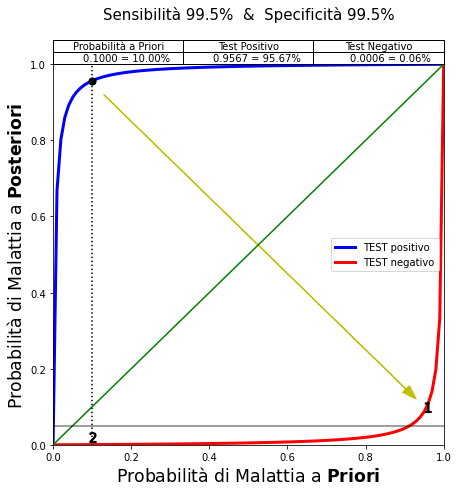
\includegraphics[width=0.5\textwidth,height=0.5\textheight,keepaspectratio]{ideale.png}
            \caption{Esempio di test "quasi" ideale.}
            \label{fig:ideale}
        \end{figure}

    
    \[ P(M|\ominus) = 0.0006 \]

    
    Notiamo come \(P(M|\ominus)\), ovvero la probabilità a posteriori di
essere malato dopo un test negativo, sia nettamente inferiore a
\(p_{\ominus}\). Dunque è sufficiente un solo test negativo per ritenere
sano un individuo di cui non si abbiano precedenti informazioni (la sua
probabilità a priori era solo la prevalenza).

\(P(M|\oplus)\), ovvero la probabilità a posteriori di essere malato
dopo un test positivo per un individuo nelle stesse condizioni, risulta
superiore al 95\% e diventa la nuova \emph{probabilità a priori} per
quel soggetto in caso di un test successivo (punto 1 sulla curva rossa).
Si può calcolare che \(P(M|\ominus)\) laddove la probabilità a priori
del soggetto non sia la prevalenza ma \(P(M)=P(M|\oplus)=95.67\%\) è
superiore al 5\% infatti

    \[
P(M|\ominus) = 1 - \frac{
P(\ominus|\overline{M})(1 - P(M|\oplus))
}{
P(\ominus|\overline{M})(1 - P(M|\oplus)) + (1 - P(\oplus|M))P(M|\oplus)
} = 0.1000
\]

    
    da cui ricaviamo che un test negativo in un individuo che abbia
precedentemente ricevuto un test positivo, non è sufficiente a ritenerlo
sano ma ne sarà necessario un altro. Si può calcolare che la probabilità
massima a priori per la quale sia sufficiente un solo test negativo per
ritenere sano l'individuo (alla condizioni poste) è pari alla
risoluzione per \(P(M)\) di

\begin{equation}\label{eq:massima1}
p_{\ominus} = 1 - P(\overline{M}|\ominus)
\end{equation}

ovvero

\begin{equation}\label{eq:massima2}
p_{\ominus} = 1 - \frac{
P(\ominus|\overline{M})(1 - P(M))
}{
P(\ominus|\overline{M})(1 - P(M)) + (1 - P(\oplus|M))P(M)
}
\end{equation}

    da cui si ricava facilmente che \(P(M)_{max} = 0.9128\).

    
    Al di sotto di questa probabilità a priori, con questi valori di
sensibilità e specificità, servirà un solo test negativo per escludere,
stabilito \(p_{\ominus}<.05\), che l'individuo sia malato.

    Notiamo anche come, a parità di sensibilità e specificità, la prevalenza
(ovvero la probabilità di malattia a priori) influisca sulla probabilità
di malattia a posteriori. Ad esempio per una malattia rara come la
Sindrome di Cushing endogena con prevalenza in Europa di un 1 caso du
26'000 \cite{cushing} ovvero

    \(P(M)=0.000038=0.0038%
\)\%, la probabilità di malattia a posteriori in seguito a test positivo
(con sensibilità e specificità di \(.995\)) sia

    
    \(P(M|\oplus)=0.0076=0.76%
\)\% dunque molto bassa anche se notevolmente superiore rispetto alla
probabilità a priori.

    
    In questo caso, a parità di sensibilità, servirebbe un test altamente
specifico, ad esempio con \(P(\ominus|\overline{M})=.9999\) col quale si
otterrebbe una probabilità a posteriori per test positivo pari a

    \(P(M|\oplus)=0.2768=27.68%
\)\%

    
    \hypertarget{sensibilituxe0-e-specificituxe0}{%
\section{Sensibilità e
Specificità}\label{sensibilituxe0-e-specificituxe0}}

    Mantenendo fissa la sensibilità a \(.995\), variamo la specificità e
viceversa

    
        \begin{figure}
        \centering
            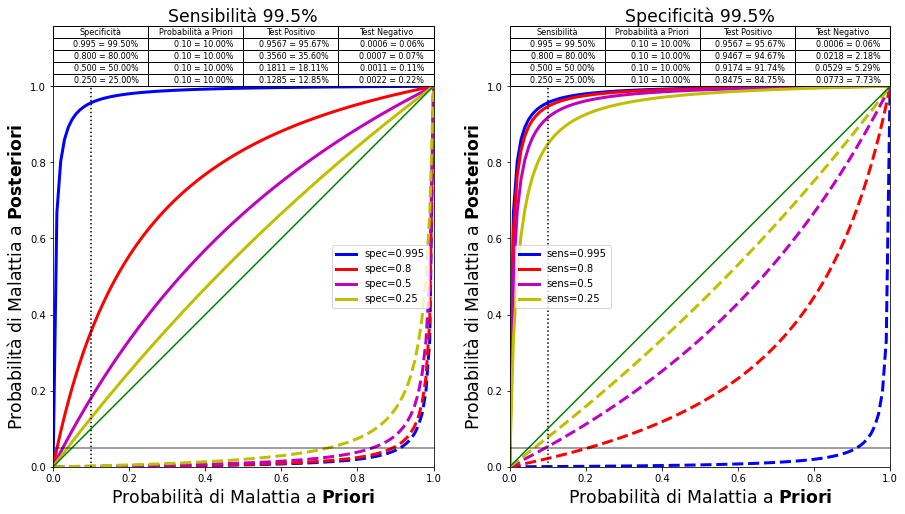
\includegraphics{sens-spec.png}
            \caption{Rapporto tra specificità e sensibilità. Le linee piene indicano $P(M|\oplus)$, le linee tratteggiate $P(M|\ominus).$}
            \label{fig:sens-spec}
        \end{figure}

    
    Notiamo come valori differenti di specificità a parità di sensibilità (o
viceversa) abbiano effetti sia sulla probabibilità a posteriori per test
positivo che per test negativo sebbene

\begin{itemize}
\tightlist
\item
  variazioni nella specificità \(P(\ominus|\overline{M})\) abbiano
  maggior effetto su \(P(M|\oplus)\)
\item
  variazioni nella sensibilità \(P(\oplus|M)\) abbiano maggior effetto
  su \(P(\overline{M}|\ominus)\)
\end{itemize}

    
        \begin{figure}
        \centering
            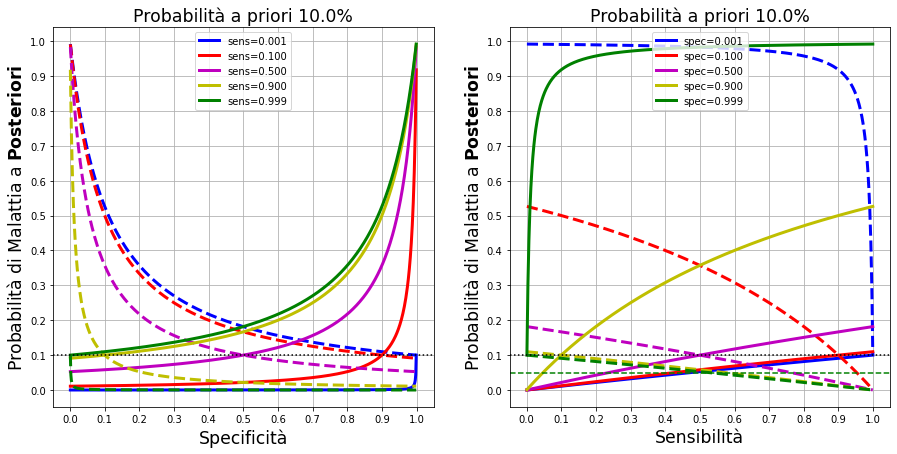
\includegraphics{sens-spec-2.png}
            \caption{Rapporto tra specificità e sensibilità. Le linee piene indicano $P(M|\oplus)$, le linee tratteggiate $P(M|\ominus).$ Si nota come sia necessario che i test abbiano determinate caratteristiche per poter essere utili.}
            \label{fig:sens-spec-2}
        \end{figure}

    
    Si nota come sensibilità e specificità siano strettamente interconnesse.
In particolare, data una probabilità di malattia a priori \(P(M)\), si
vuole che un test abbia

\begin{itemize}
\tightlist
\item
  una probabilità di malattia a posteriori dato test positivo almeno
  \(P(M|\oplus)>P(M)\)
\item
  una probabilità di malattia a posteriori dato test negativo almeno
  \(P(M|\ominus)<P(M)\)
\end{itemize}

Per trovare i minimi requisiti di un test diagnostico dunque, data la
probabilità di malattia a priori, si può risolvere il sistema a due
equazioni

\[
\left\{\begin{matrix}
P(M|\oplus) > P(M) \\
P(M|\ominus) < P(M)
\end{matrix}\right.
\]

ma avendo stabilito \(p_{\ominus}<.05\) per \(P(M|\ominus)\) si può
anche assumere \(p_{\oplus}>.5\) per \(P(M|\oplus)\) ovvero che la
probabilità di malattia a posteriori dato test positivo sia almeno
superiore al 50\% come requisito minimo e \(p_{\oplus}>.9\) (ovver
superiore al 90\%) come requisito ottimale.

\[
\left\{\begin{matrix}
P(M|\oplus) > p_{\oplus} \\
P(M|\ominus) < p_{\ominus}
\end{matrix}\right.
\]

    
        \begin{figure}
        \centering
            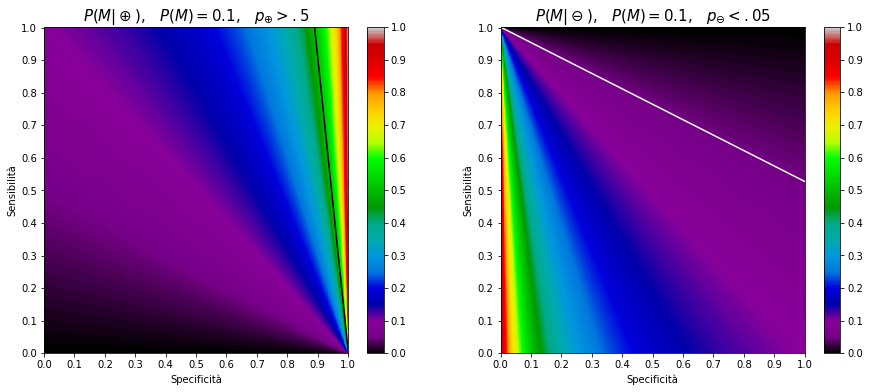
\includegraphics{requisitimatrice10.png}
            \caption{Requisiti per $P(M)=.1$. L'area a destra della linea nera nell'immagine di sinistra è il requisito minimo per $P(M|\oplus)>.5$  e a destra della linea bianca i requisito ideale per $p(M|\oplus)>.9$. L'area a destra della linea bianca nell'immagine di destra è il requisito minimo per $P(M|\ominus)<.05$.}
            \label{fig:requisitimatrice10}
        \end{figure}

    
    
        \begin{figure}
        \centering
            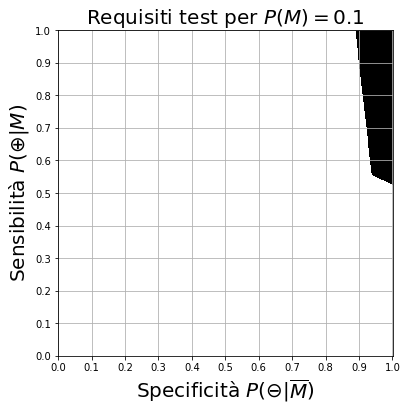
\includegraphics[width=0.5\textwidth,height=0.5\textheight,keepaspectratio]{requisiti10.png}
            \caption{L'area nera indica i requisiti minimi necessari $P(M|\oplus)>.5$ e $P(M|\ominus)<.05$ per un test con $P(M)=.1$. L'area azzurra i requisiti ottimali per $P(M|\oplus)>.9$.}
            \label{fig:requisiti10}
        \end{figure}

    
    \hypertarget{covid-19-e-tamponi-naso-faringei}{%
\section{COVID-19 e tamponi
naso-faringei}\label{covid-19-e-tamponi-naso-faringei}}

Studi recenti suggeriscono che i tamponi naso-faringei usati per la
diagnosi di COVID-19 (RT-PCR SARS-CoV-2 RNA test) abbiano sensibilità
\(P(\oplus|M)=0.777\) e specificità di \(P(\ominus|\overline{M})=0.988\)
\cite{padhye2020reconstructed} e che la prevalenza di COVID-19 in Italia
(in fase pandemica) sia circa pari a \(P(M)=0.13\)
\cite{ceylan2020estimation} \cite{vollmer2020sub}
\cite{flaxman2020report}.

Verifichiamo che il test abbia i requisiti richiesti (figura
\(\ref{fig:requisiti13}\)): il punto giallo indica i parametri di
sensibilità e specificità dei test in esame per \(P(M)=.13\), i test
hanno quindi caratteristiche ottimali.

    
        \begin{figure}
        \centering
            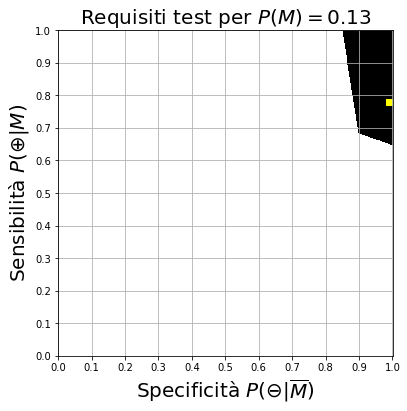
\includegraphics[width=0.5\textwidth,height=0.5\textheight,keepaspectratio]{requisiti13.png}
            \caption{L'area nera indica i requisiti necessari $P(M|\oplus)>.5$ e $P(M|\ominus)<.05$ per un test con $P(M)=.13$ (azzurra ottimali per $P(M|\oplus)>.9$). Il punto giallo indica i parametri di sensibilità e specificità dei test RT-PCR SARS-CoV-2 RNA test per COVID-19: sensibilità $P(\oplus|M)=0.777$ e specificità di $P(\ominus|\overline{M})=0.988$}
            \label{fig:requisiti13}
        \end{figure}

    
    Vediamo come si modificano le curve delle probabilità a posteriori
impostando questi tre parametri (figura \(\ref{fig:covid}\)).

    
        \begin{figure}
        \centering
            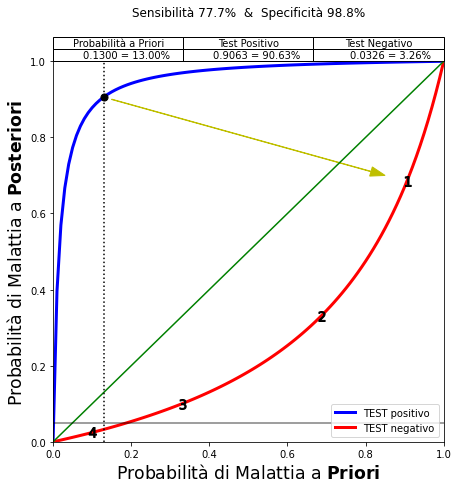
\includegraphics[width=0.5\textwidth,height=0.5\textheight,keepaspectratio]{covid.png}
            \caption{Probabilità di malattia COVID-19 a posteriori per test RT-PCR SARS-CoV-2 RNA.}
            \label{fig:covid}
        \end{figure}

    
    Anche in questo caso dunque è sufficiente un test negativo per ritenere
sano un soggetto su cui non si abbiano precedenti informazioni.

    \[
P(M|\ominus) = 0.0326 < p_{\ominus} = 0.05
\]

    
    Se invece un soggetto risultasse positivo (punto nero in figura
\(\ref{fig:covid}\)), la sua probabilità di essere malato passerebbe da
\(0.13\) (prevalenza stimata di COVID-19 in Italia in fase pandemica) a

    \[
P(M|\oplus) = 0.9063 > p_{\oplus} = .5
\]

    
    Vediamo quindi la probabilità a posteriori per test negativo
\(P(M|\ominus)\) con la probabilità a priori di un soggetto
precedentemente risultato positivo (punto 1 in figura
\(\ref{fig:covid}\))

    \[
P(M|\ominus)_1 = 1 - \frac{
P(\ominus|\overline{M})(1 - 0.9063)
}{
P(\ominus|\overline{M})(1 - 0.9063) + (1 - P(\oplus|M))0.9063
} = 0.6859
\]

    
    Dunque un tampone negativo non è sufficiente, il soggetto ha ancora
un'elevata probabilità di essere infetto, supponiamo che ne venga fatto
un secondo (punto 2 in figura \(\ref{fig:covid}\))

    \[
P(M|\ominus)_1 = 1 - \frac{
P(\ominus|\overline{M})(1 - 0.6859)
}{
P(\ominus|\overline{M})(1 - 0.6859) + (1 - P(\oplus|M))0.6859
} = 0.3302
\]

Ancora superiore, \(33.02%
\)\% di probabilità di essere infetto non è accettabile per ritenere
guarito il paziente. Effettuiamo un terzo test (punto 3 in figura
\(\ref{fig:covid}\))

    
    \[
P(M|\ominus)_1 = 1 - \frac{
P(\ominus|\overline{M})(1 - 0.3302)
}{
P(\ominus|\overline{M})(1 - 0.3302) + (1 - P(\oplus|M))0.3302
} = 0.1001
\]

\(10.01%
\)\% nuovamente superiore a \(p_{\ominus}\), dunque effettuiamo un
quarto test (punto 4 in figura \(\ref{fig:covid}\))

    
    \[
P(M|\ominus)_1 = 1 - \frac{
P(\ominus|\overline{M})(1 - 0.1001)
}{
P(\ominus|\overline{M})(1 - 0.1001) + (1 - P(\oplus|M))0.1001
} = 0.0245
\]

\(2.45%
\)\% di probabilità di essere infetto è un valore che possiamo ritenere
accettabile per considerarlo sano. Servirebbero quindi quattro tamponi
nasofaringei negativi per escludere la possibilità che un soggetto
precedentemente risultato positivo per COVID-19 sia considerabile
attualmente guarito \(P(M|\ominus)<.05\).

    
    Calcolando in questo caso la massima probabilità a priori \(P(M)_{max}\)
data la quale sia sufficiente un solo tampone negativo per considerare
sano il soggetto, otteniamo

    \[P(M)_{max} = 0.1891\]

ovvero per probabilità a priori \(P(M^*)>18.91%
\)\% servirà sicuramente più di un tampone.

    
    \hypertarget{covid-19-e-test-sierologici-rapidi}{%
\section{COVID-19 e test sierologici
rapidi}\label{covid-19-e-test-sierologici-rapidi}}

    Nella cosiddetta ``fase-2'' verranno probabilmente utilizzati test
sierologici rapidi (\textbf{RDT}) \cite{rdtdiagram}.

Specificità e sensibilità dichiarate sono piuttosto variabili in questo
tipo di test \cite{rdt}, vedi tabella \(\ref{tab:rdtall}\) e
\(\ref{tab:rdtstats}\).

    
\begin{table}
  \begin{center}
    \caption{Specificità e sensibilità di alcuni test rapidi RDT}
    \label{tab:rdtall}
    \begin{tabular}{c|c|c|}
        & specificità & sensibilità \\
        \toprule
        1 & 0.956 & 0.938\\ \midrule 2 & 0.99 & 0.9735\\ \midrule 3 & 1.0 & 0.9255\\ \midrule 4 & 0.97 & 0.82\\ \midrule 5 & 0.987 & 1.0\\ \midrule 6 & 0.994 & 0.969\\ \midrule 7 & 0.9063 & 0.886\\ \midrule 8 & 0.923 & 0.841\\ \midrule 9 & 0.955 & 0.87\\ \midrule 10 & 0.967 & 0.91\\ \midrule 11 & 0.96 & 0.82\\ \midrule 12 & 1.0 & 0.95\\ \midrule 13 & 1.0 & 0.931\\ \midrule 14 & 0.991 & 0.931\\ \midrule 15 & 0.977 & 0.934\\ \midrule 16 & 0.9935 & 0.9585
    \end{tabular}
  \end{center}
\end{table}
        

    
    
        \begin{figure}
        \centering
            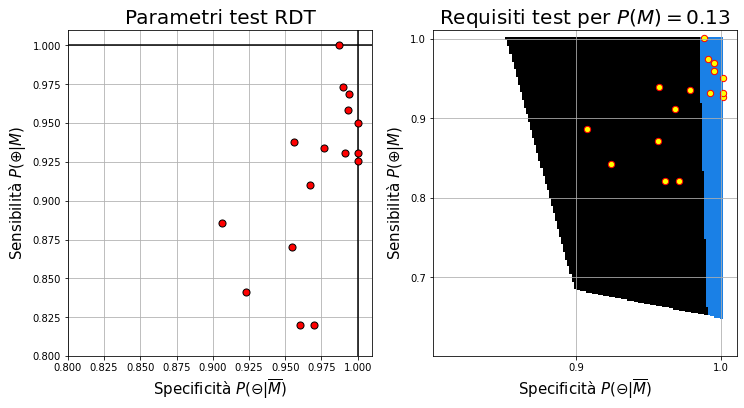
\includegraphics{requisitiRDT.png}
            \caption{L'area nera indica i requisiti necessari $P(M|\oplus)>.5$ e $P(M|\ominus)<.05$ per un test con $P(M)=.13$. Il punti gialli indicano i parametri di sensibilità e specificità dei test RDT per COVID-19.}
            \label{fig:requisitiRDT}
        \end{figure}

    
    I parametri di specificità e sensibilità sono nell'area dei parametri
minimi accettabili stabiliti in precedenza \(\ref{fig:requisitiRDT}\) e
per metà dei test i parametri risultano ottimali.

Verifichiamo le probabilità a posteriori per i test con minor
sensibilità o specificità (figura \(\ref{fig:covidrdtpeggio}\)) e con
maggior sensibilità o specificità (figura \(\ref{fig:covidrdtmeglio}\)).

    
\begin{table}
  \begin{center}
    \caption{Specificità e sensibilità dei test rapidi RDT}
    \label{tab:rdtstats}
    \begin{tabular}{c|c|c|c|c|c|}
        & n & mean & std & min & max \\
        \toprule
        Sensibilità & 16 & 0.916 & 0.055
        & 0.820 & 1.000 \\
        \midrule
        Specificità & 16 & 0.973 & 0.028
        & 0.906 & 1.000 \\
    \end{tabular}
  \end{center}
\end{table}
        

    
    
        \begin{figure}
        \centering
            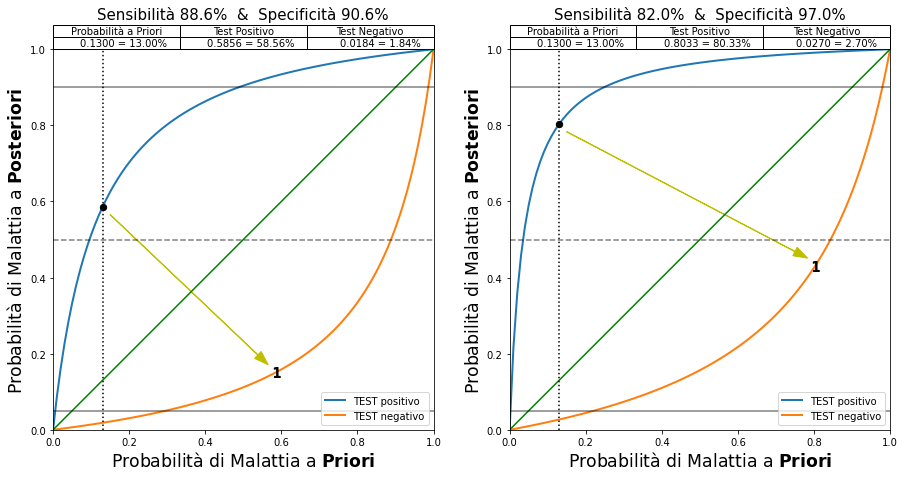
\includegraphics{covidrdtpeggio.png}
            \caption{Probabilità di malattia COVID-19 a posteriori per test RDT per le peggiori sensibilità o specificità.}
            \label{fig:covidrdtpeggio}
        \end{figure}

    
    
        \begin{figure}
        \centering
            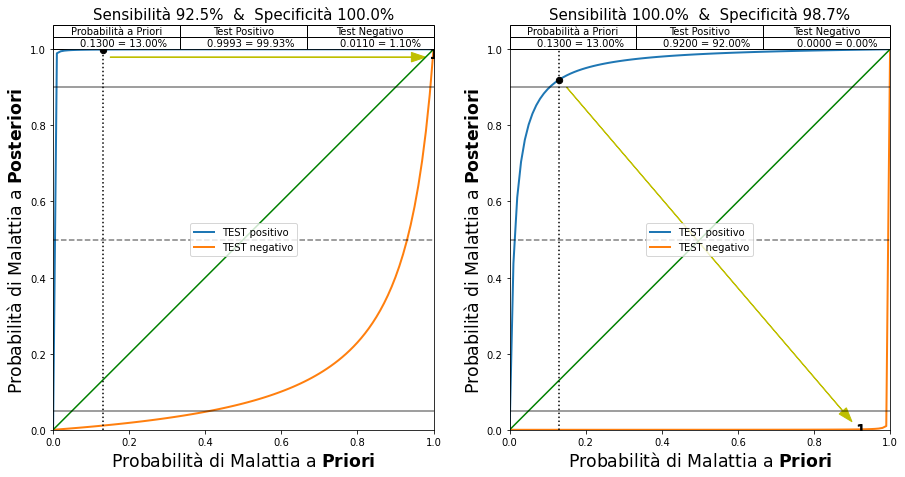
\includegraphics{covidrdtmeglio.png}
            \caption{Probabilità di malattia COVID-19 a posteriori per test RDT con miglior specificità o sensibilità.}
            \label{fig:covidrdtmeglio}
        \end{figure}

    
    
        \begin{figure}
        \centering
            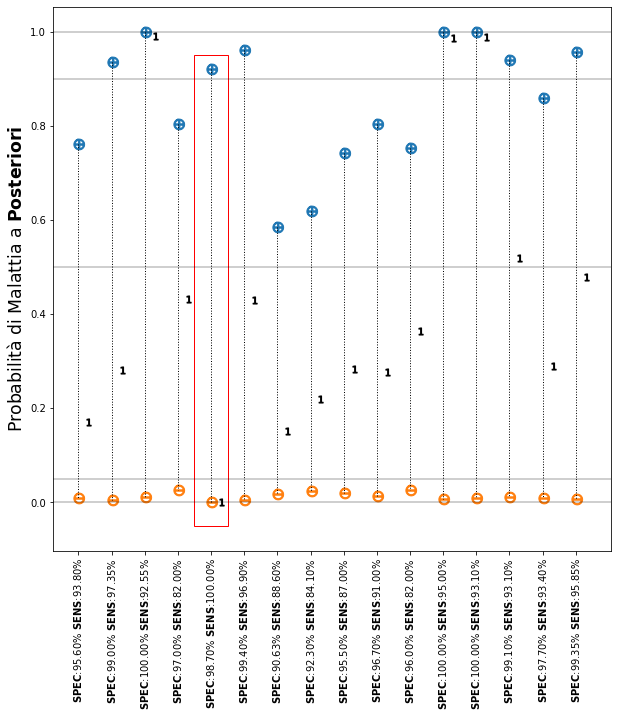
\includegraphics[width=0.5\textwidth,height=0.5\textheight,keepaspectratio]{allrdt.png}
            \caption{Probabilità di malattia a posteriori per i test RDT.}
            \label{fig:allrdt}
        \end{figure}

    
    Tutti i test RDT sono dunque utili per escludere la probabilità a
posteriori di malattia in caso di test negativi \(P(M|\ominus)\) su
individui di cui non si abbiano precedenti informazioni, figura
\(\ref{fig:allrdt}\), ma molti test presentano probabilità a posteriori
in caso di test positivi \(P(M|\oplus)\) molto al di sotto dei parametri
ottimali \(p_{\oplus}=.90\). Tra i test con \(P(M|\oplus)>.90\) è
probabilmente preferibile il quinto da sinista in figura
\(\ref{fig:allrdt}\) (e grafico a destra in figura
\(\ref{fig:covidrdtmeglio}\)) con specificità 98.7\% e sensibilità 100\%
dato che è sufficiente un solo test in tutti i casi, anche per escludere
la probabilità a posteriori di malattia in un soggetto precedentemente
risultato positivo.


    % Add a bibliography block to the postdoc
    
    
\bibliographystyle{IEEEtran}
\bibliography{IEEEabrv,biblio}

    
\end{document}
